\UseRawInputEncoding
\documentclass[hyperref]{labbook}
\usepackage{hyperref}
\usepackage[utf8]{inputenc}

\usepackage{graphicx}
\begin{document}
\labday{28.12.2020}
\experiment[before]{Measurement of germ content before and after CleanAir use}
\subexperiment{Material}
\begin{itemize}
\item agar plates (Servoplate C3 10413 Nährböden (agars), Sabouraud 2\% Glucose Agar (20-er Pack))
\begin{itemize}
\item pepton: 10g/l
\item D(+) glucose: 20g/l
\item agar: 17g/l
\end{itemize}
\item Kreppband
\end{itemize}
\subexperiment{Baseline}
\begin{itemize}
\item office room - measurements?
\item meeting room table 
\item 6 chairs around table
\item 4 chairs at short wall
\item 1 pot plant
\item window façade at the opposite the wall where CleanAir device was placed
\end{itemize}
\subexperiment{Experimental setup}
\begin{itemize}
\item 4 different distances
\item duplicates
\item incubation time: 47-48min
\end{itemize}
\begin{figure}[h]
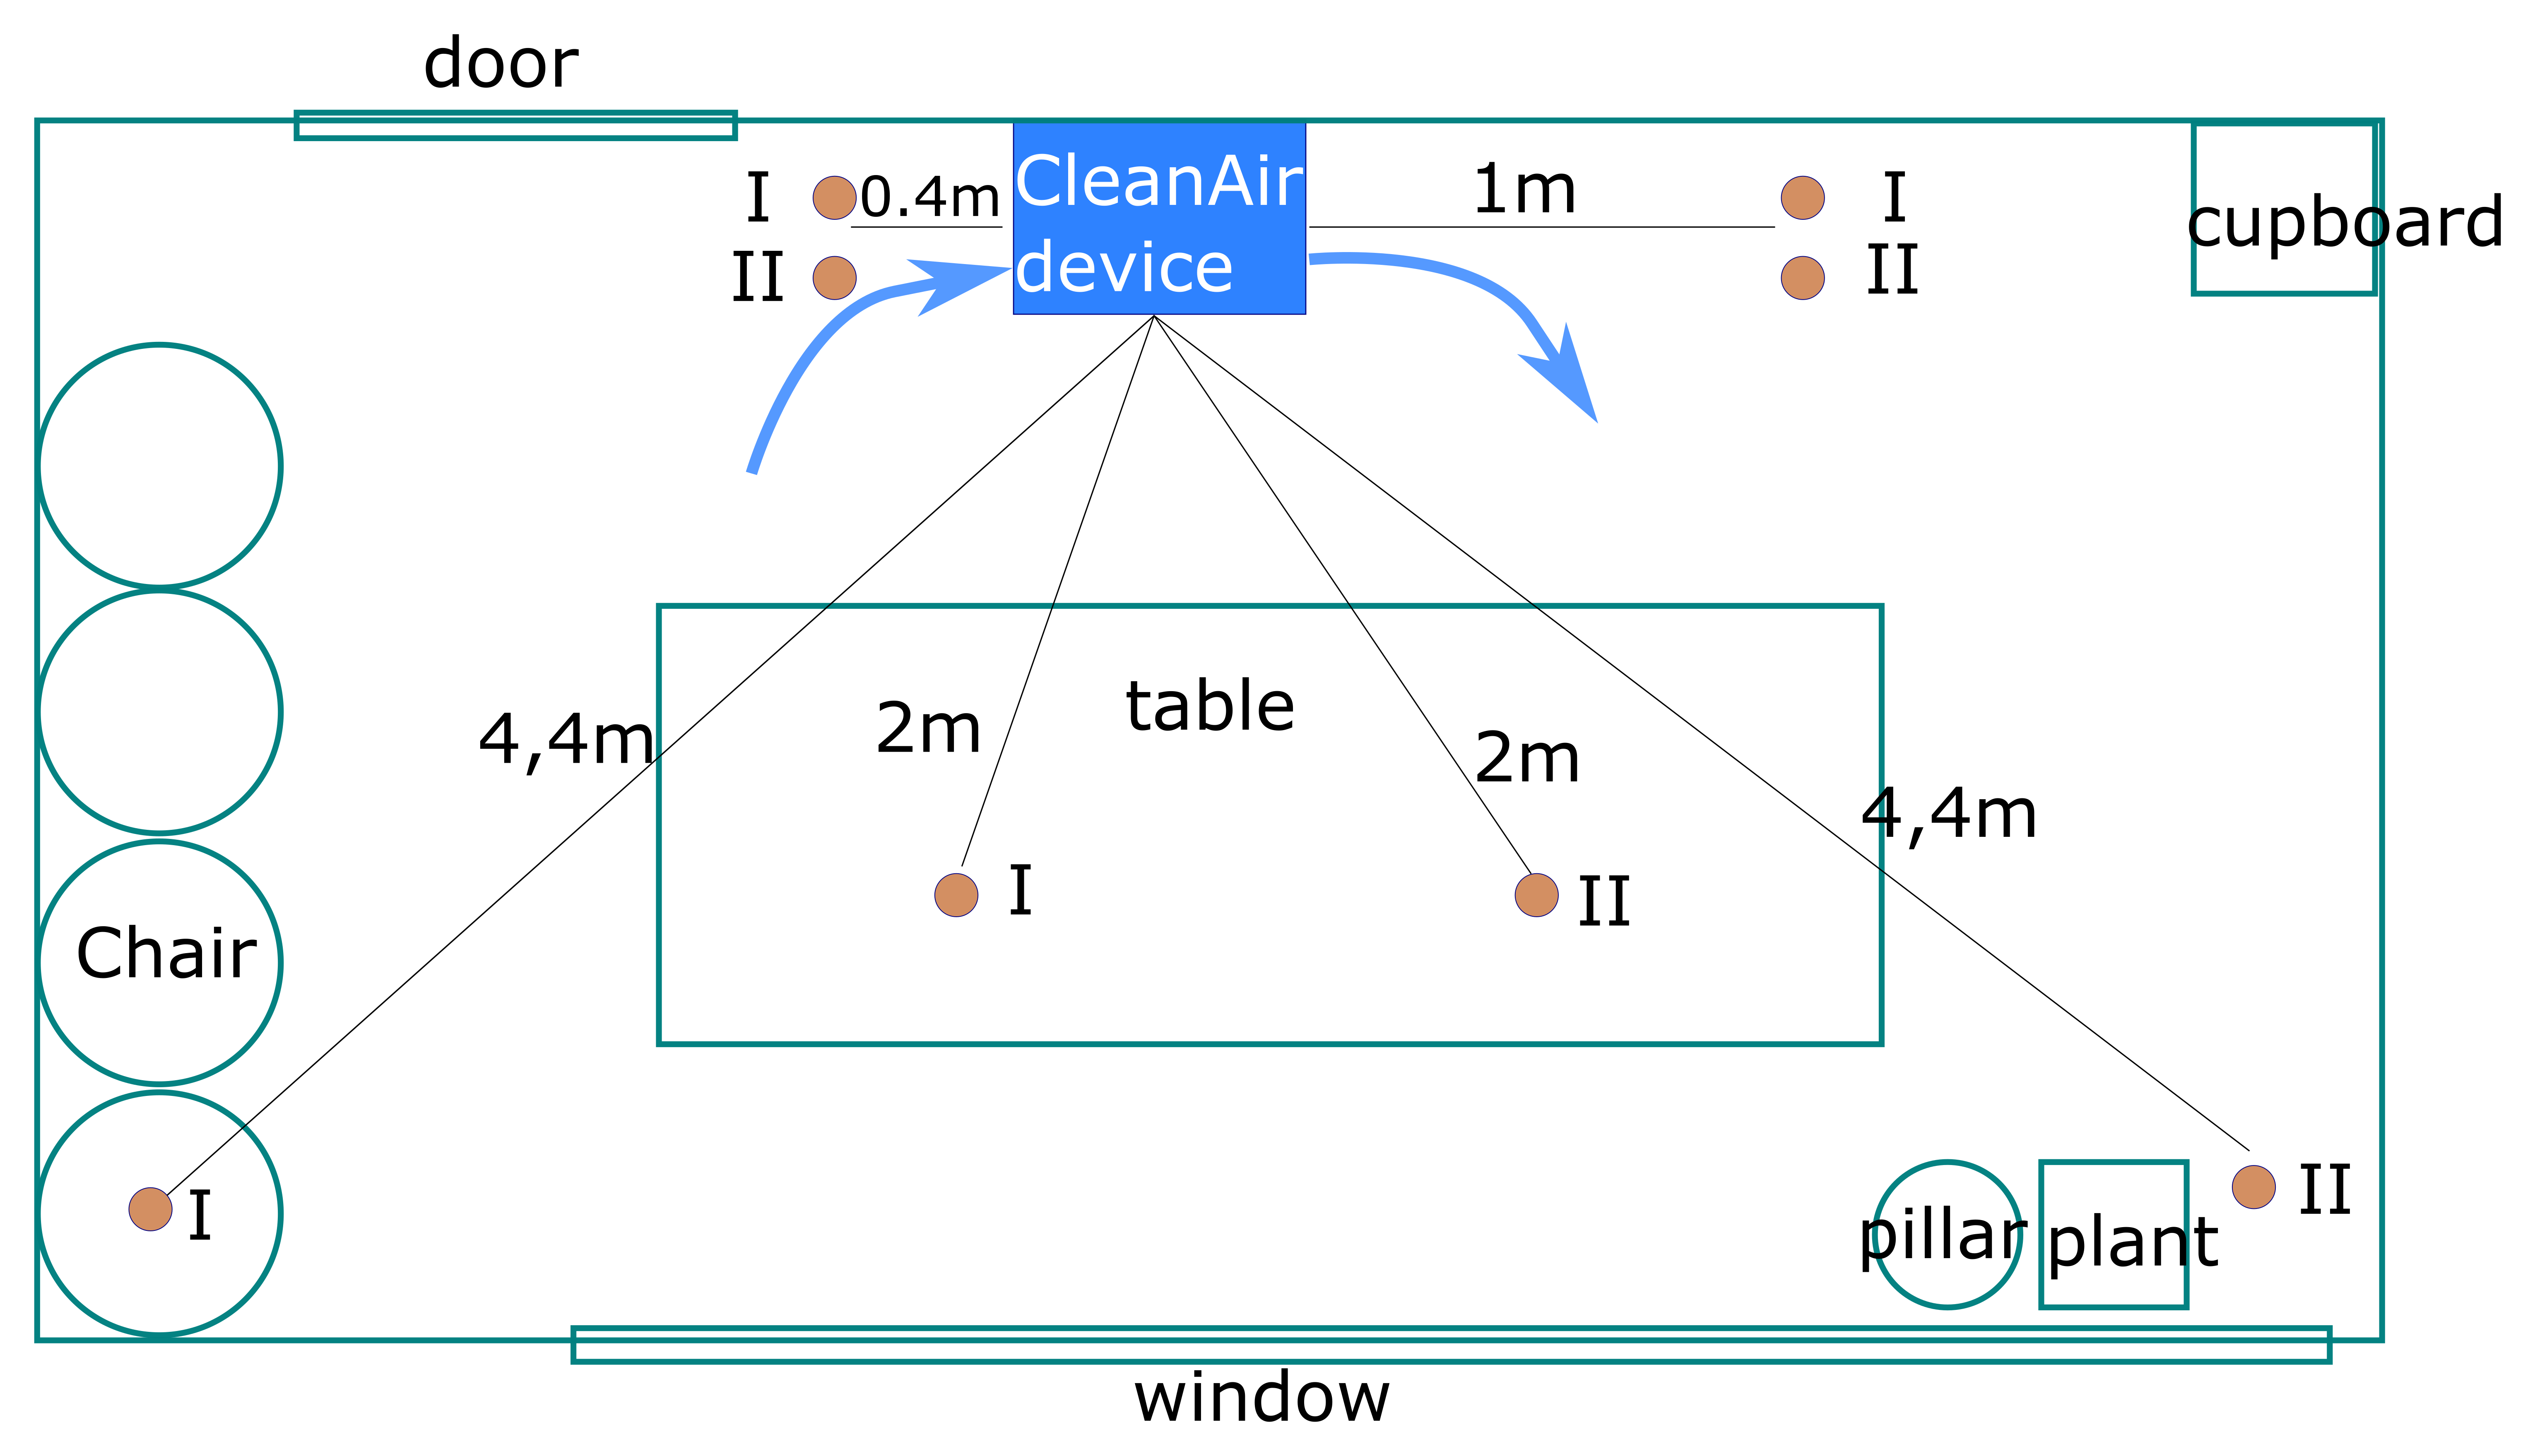
\includegraphics[scale=0.28]{cleanair_experiment_schema}
\caption{Schema of office room with the approximate placing of the table, chairs and plant as well as the placing of the CleanAir device. Air flow direction is indicated by the arrows. Agar plates are depicted as brown circles.}
\end{figure}
\begin{table}[h!]
\begin{tabular}{|lll|}\hline
Distance from CleanAir  & height from ground & labelling\\\hline
0,4m from suction area & 0m & 28.12., 0,4m, front, before, 1 \\
0,4m from suction area & 0m & 28.12., 0,4m, before, 2 \\
1m from emitting area & 0m & 28.12., 1m, before, back, 1\\
1m from emitting area & 0m & 28.12., 1m, before, back, 2\\
2m & 0,76m & 28.12., 2m, before, 1\\
2m & 0,76m & 28.12., 2m, before, 2\\
4,4m & 0,49m & 28.12., 4,4m, before, 1\\
4,4m & 0m & 28.12., 4,4m, before, 2\\\hline
0,4m from suction area & 0m & 28.12., 0,4m, front, after, 1 \\
0,4m from suction area & 0m & 28.12., 0,4m, after, 2 \\
1m from emitting area & 0m & 28.12., 1m, after, back, 1\\
1m from emitting area & 0m & 28.12., 1m, after, back, 2\\
2m & 0,76m & 28.12., 2m, after, 1\\
2m & 0,76m & 28.12., 2m, after, 2\\
4,4m & 0,49m & 28.12., 4,4m, after, 1\\
4,4m & 0m & 28.12., 4,4m, after, 2\\\hline
\end{tabular}
\end{table}

\subexperiment{Description}
The office was out of use for one day before starting the experiment. The door was open beforehand. The CleanAir device was placed in the middle of the long wall of the office but was not turned on. Distances were marked using a tape to ensure that before and after measurements are taken from the same location. Plates were placed at the indicated distances from the CleanAir device. Plates were left open for the time of incubation (48min, room temperature). The door was closed during incubation. Starting time of the incubation was 9:56 am, incubation was finished at 10:43 am. The plates were then sealed with tape.\\
The CleanAir device was turned on for 38min at maximum power. The door was closed during air cleaning. (Estimated air turn over rate?)\\
Plates were placed at the indicated distances, the ClearAir device was turned off and plates were left open. Incubation was at room temperature and started at 11:21 am and ended at 12:09 pm. Plates were sealed with tape.\\
Plates were left at room temperature until colonies are formed. (to be continued.)

\begin{figure*}[h!]
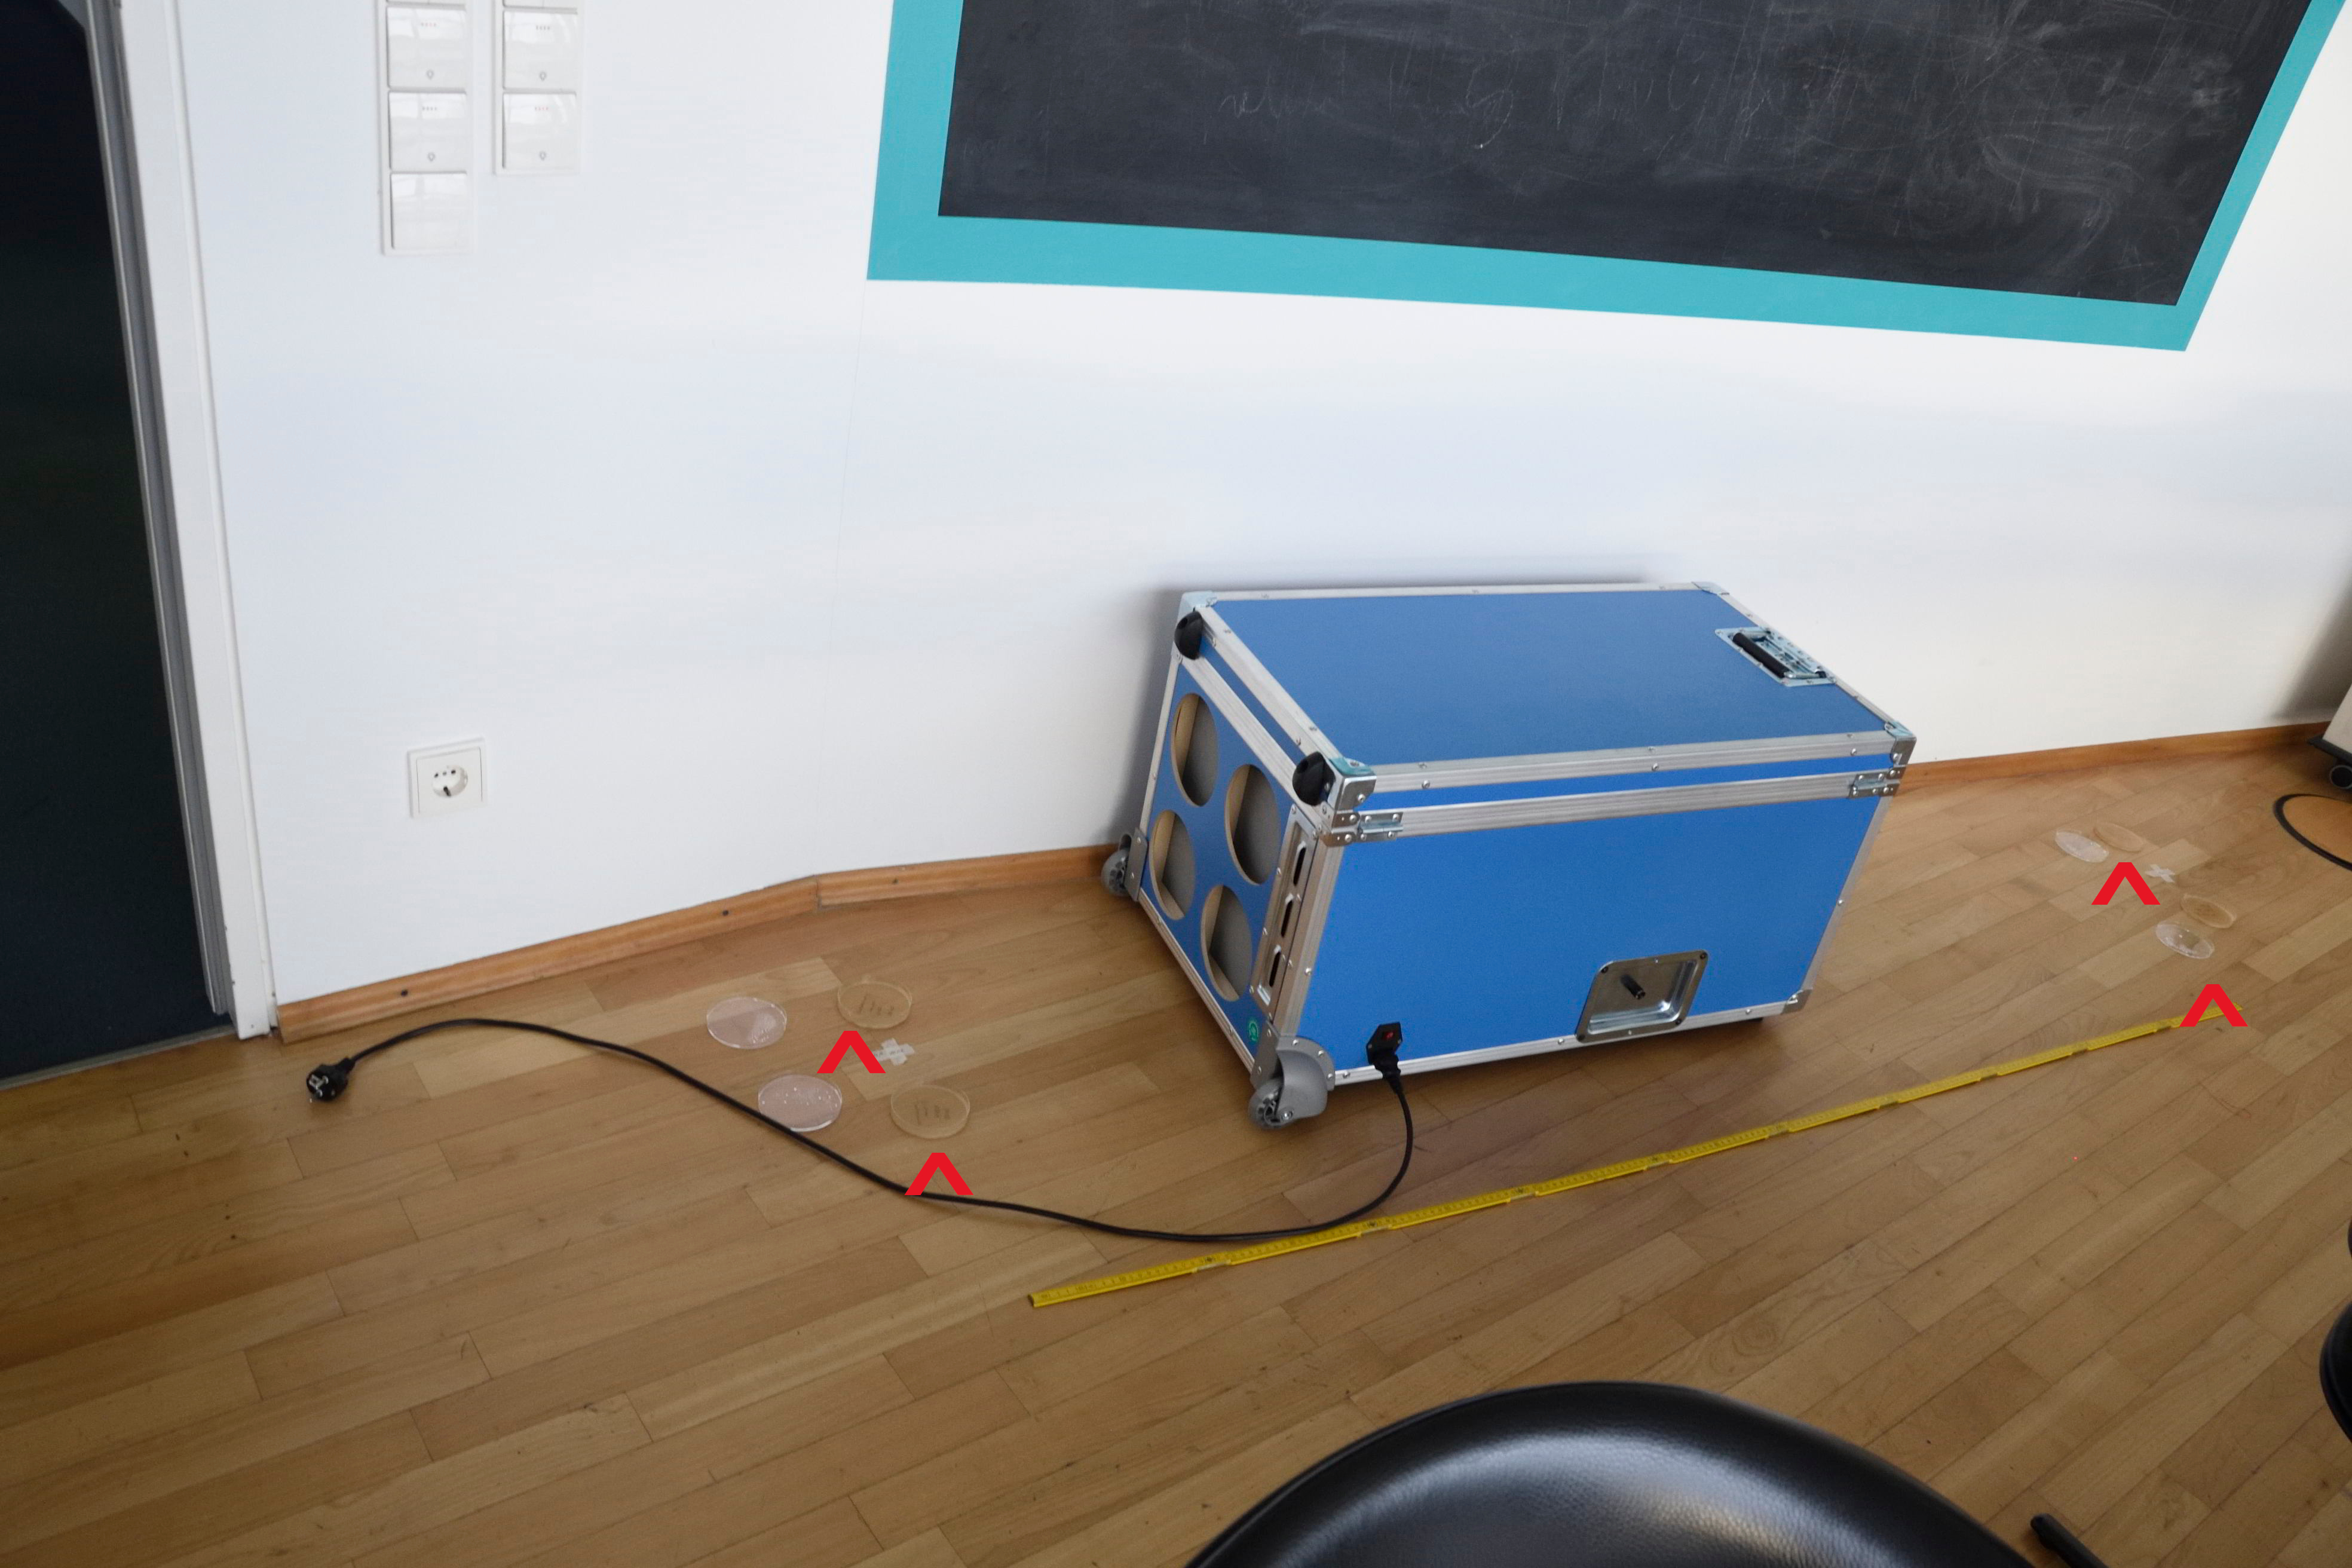
\includegraphics[scale=0.05]{_DSC7617}\hfill
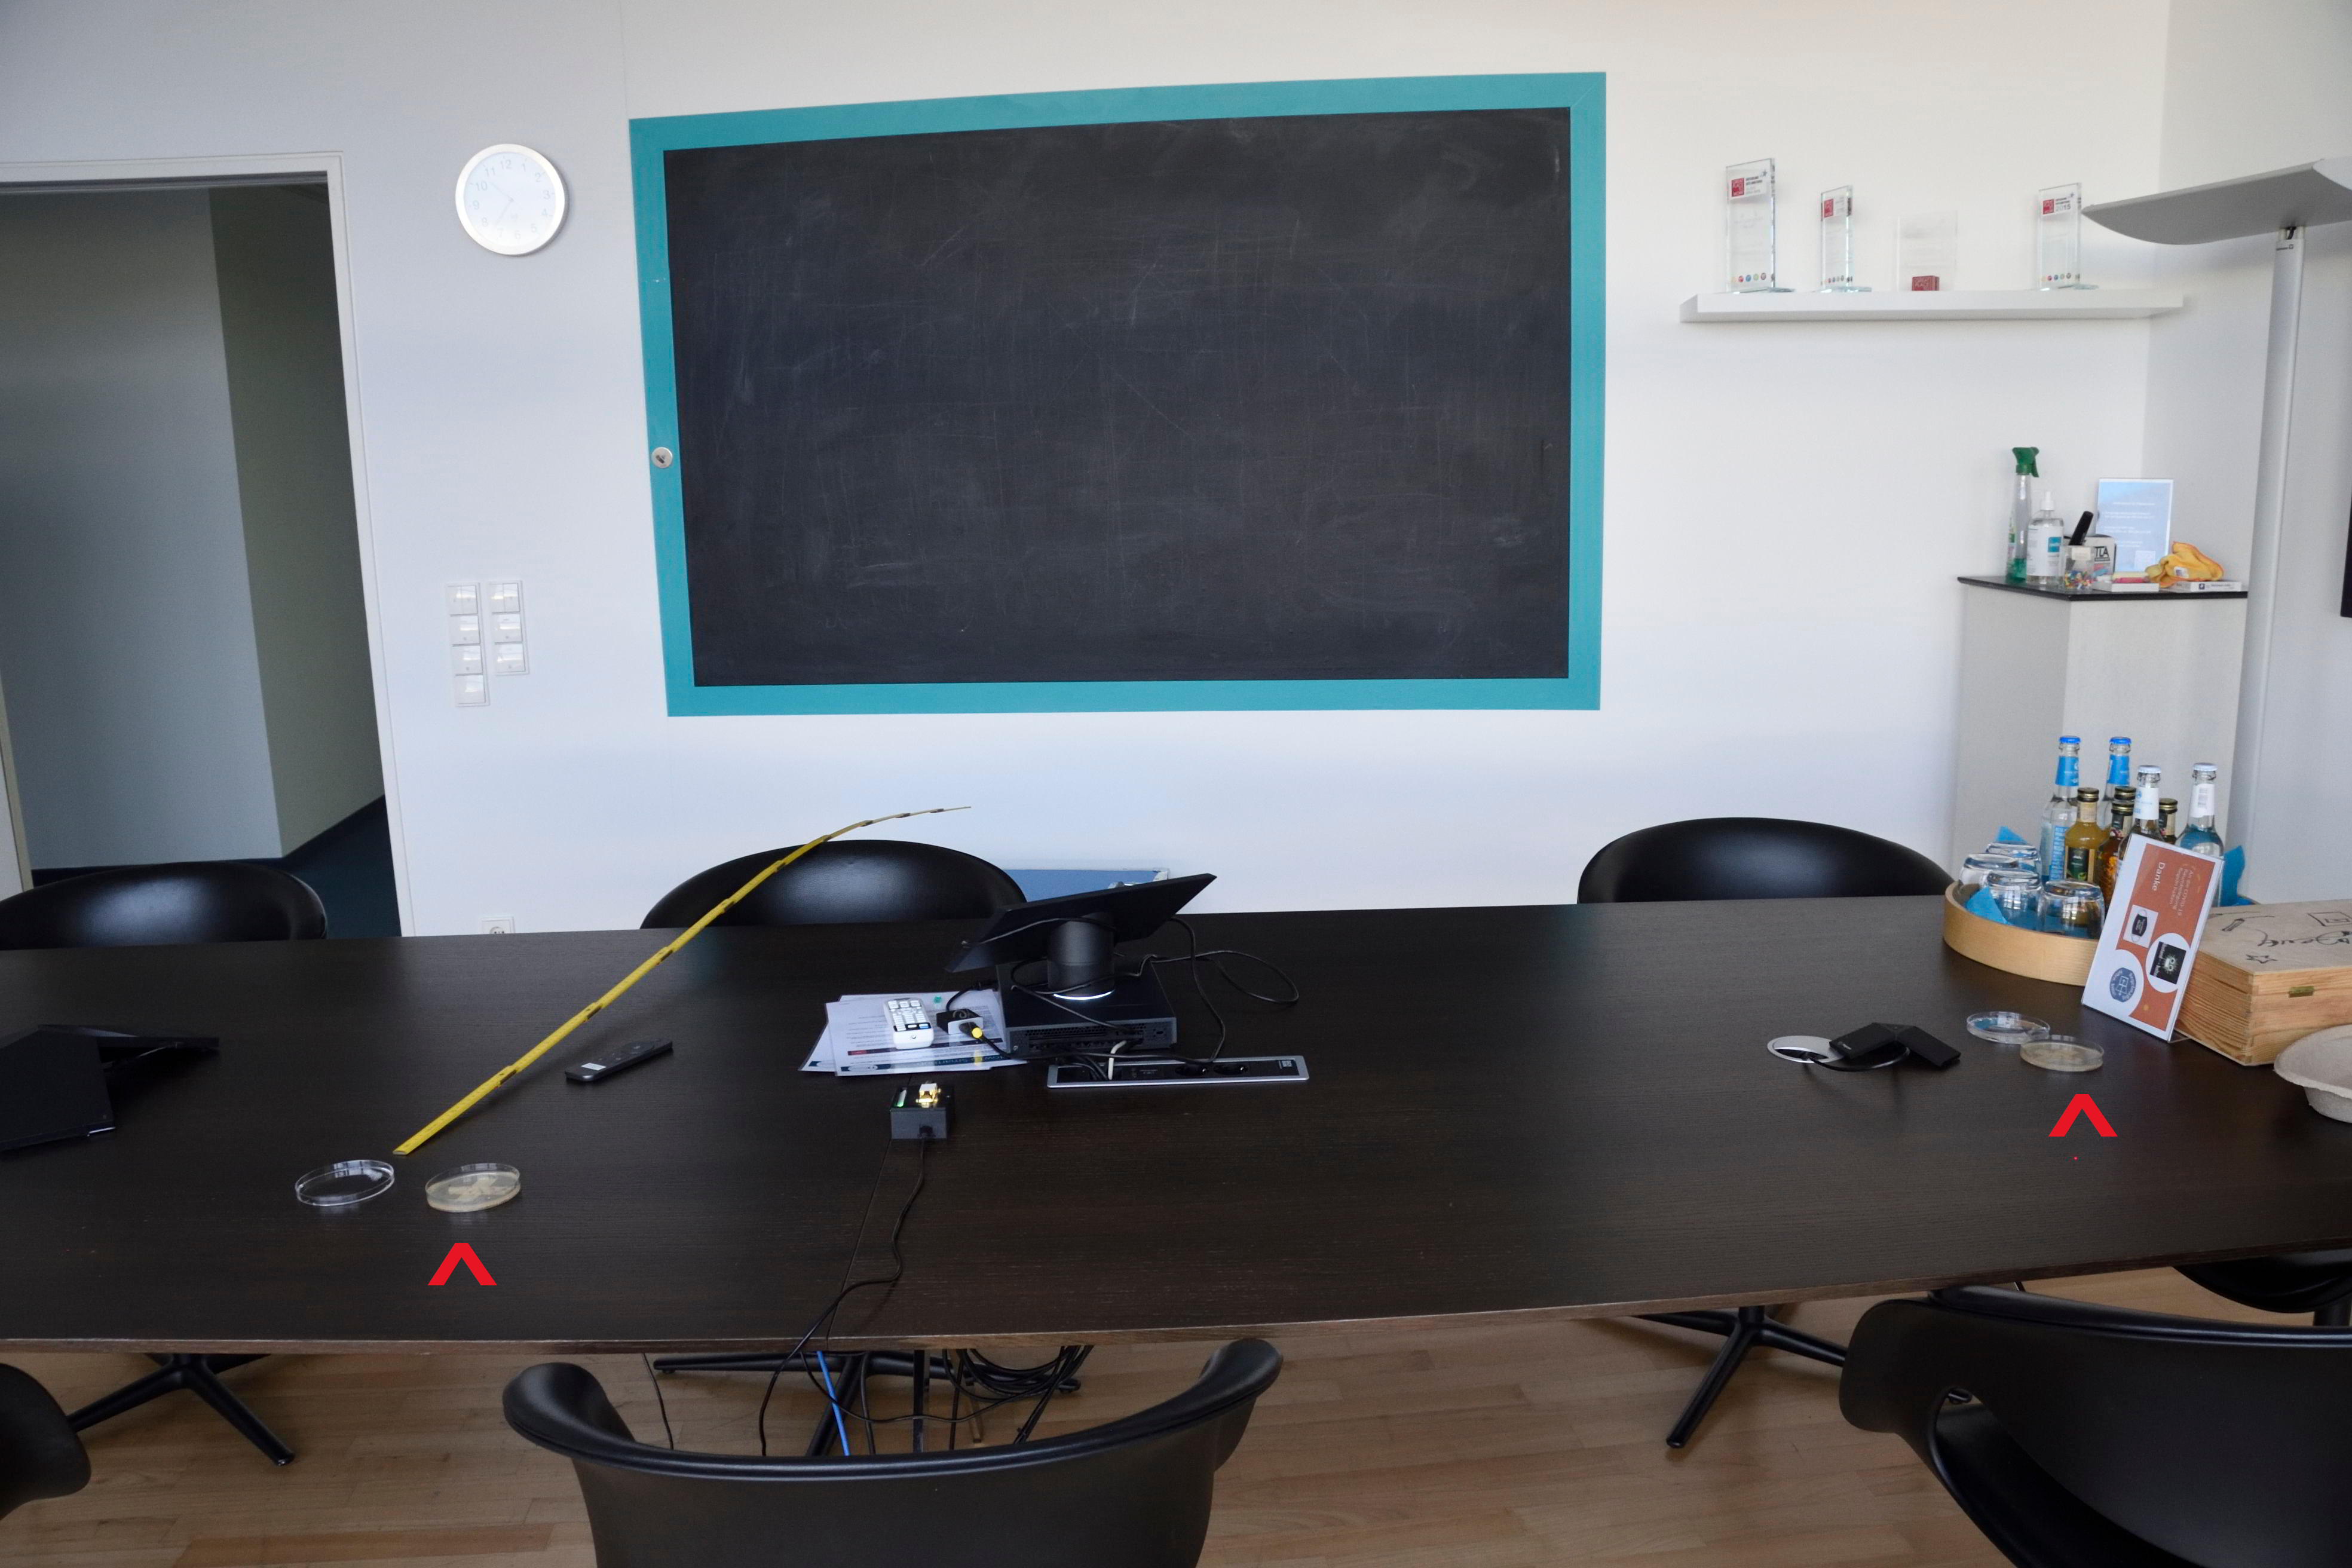
\includegraphics[scale=0.05]{_DSC7622}\\
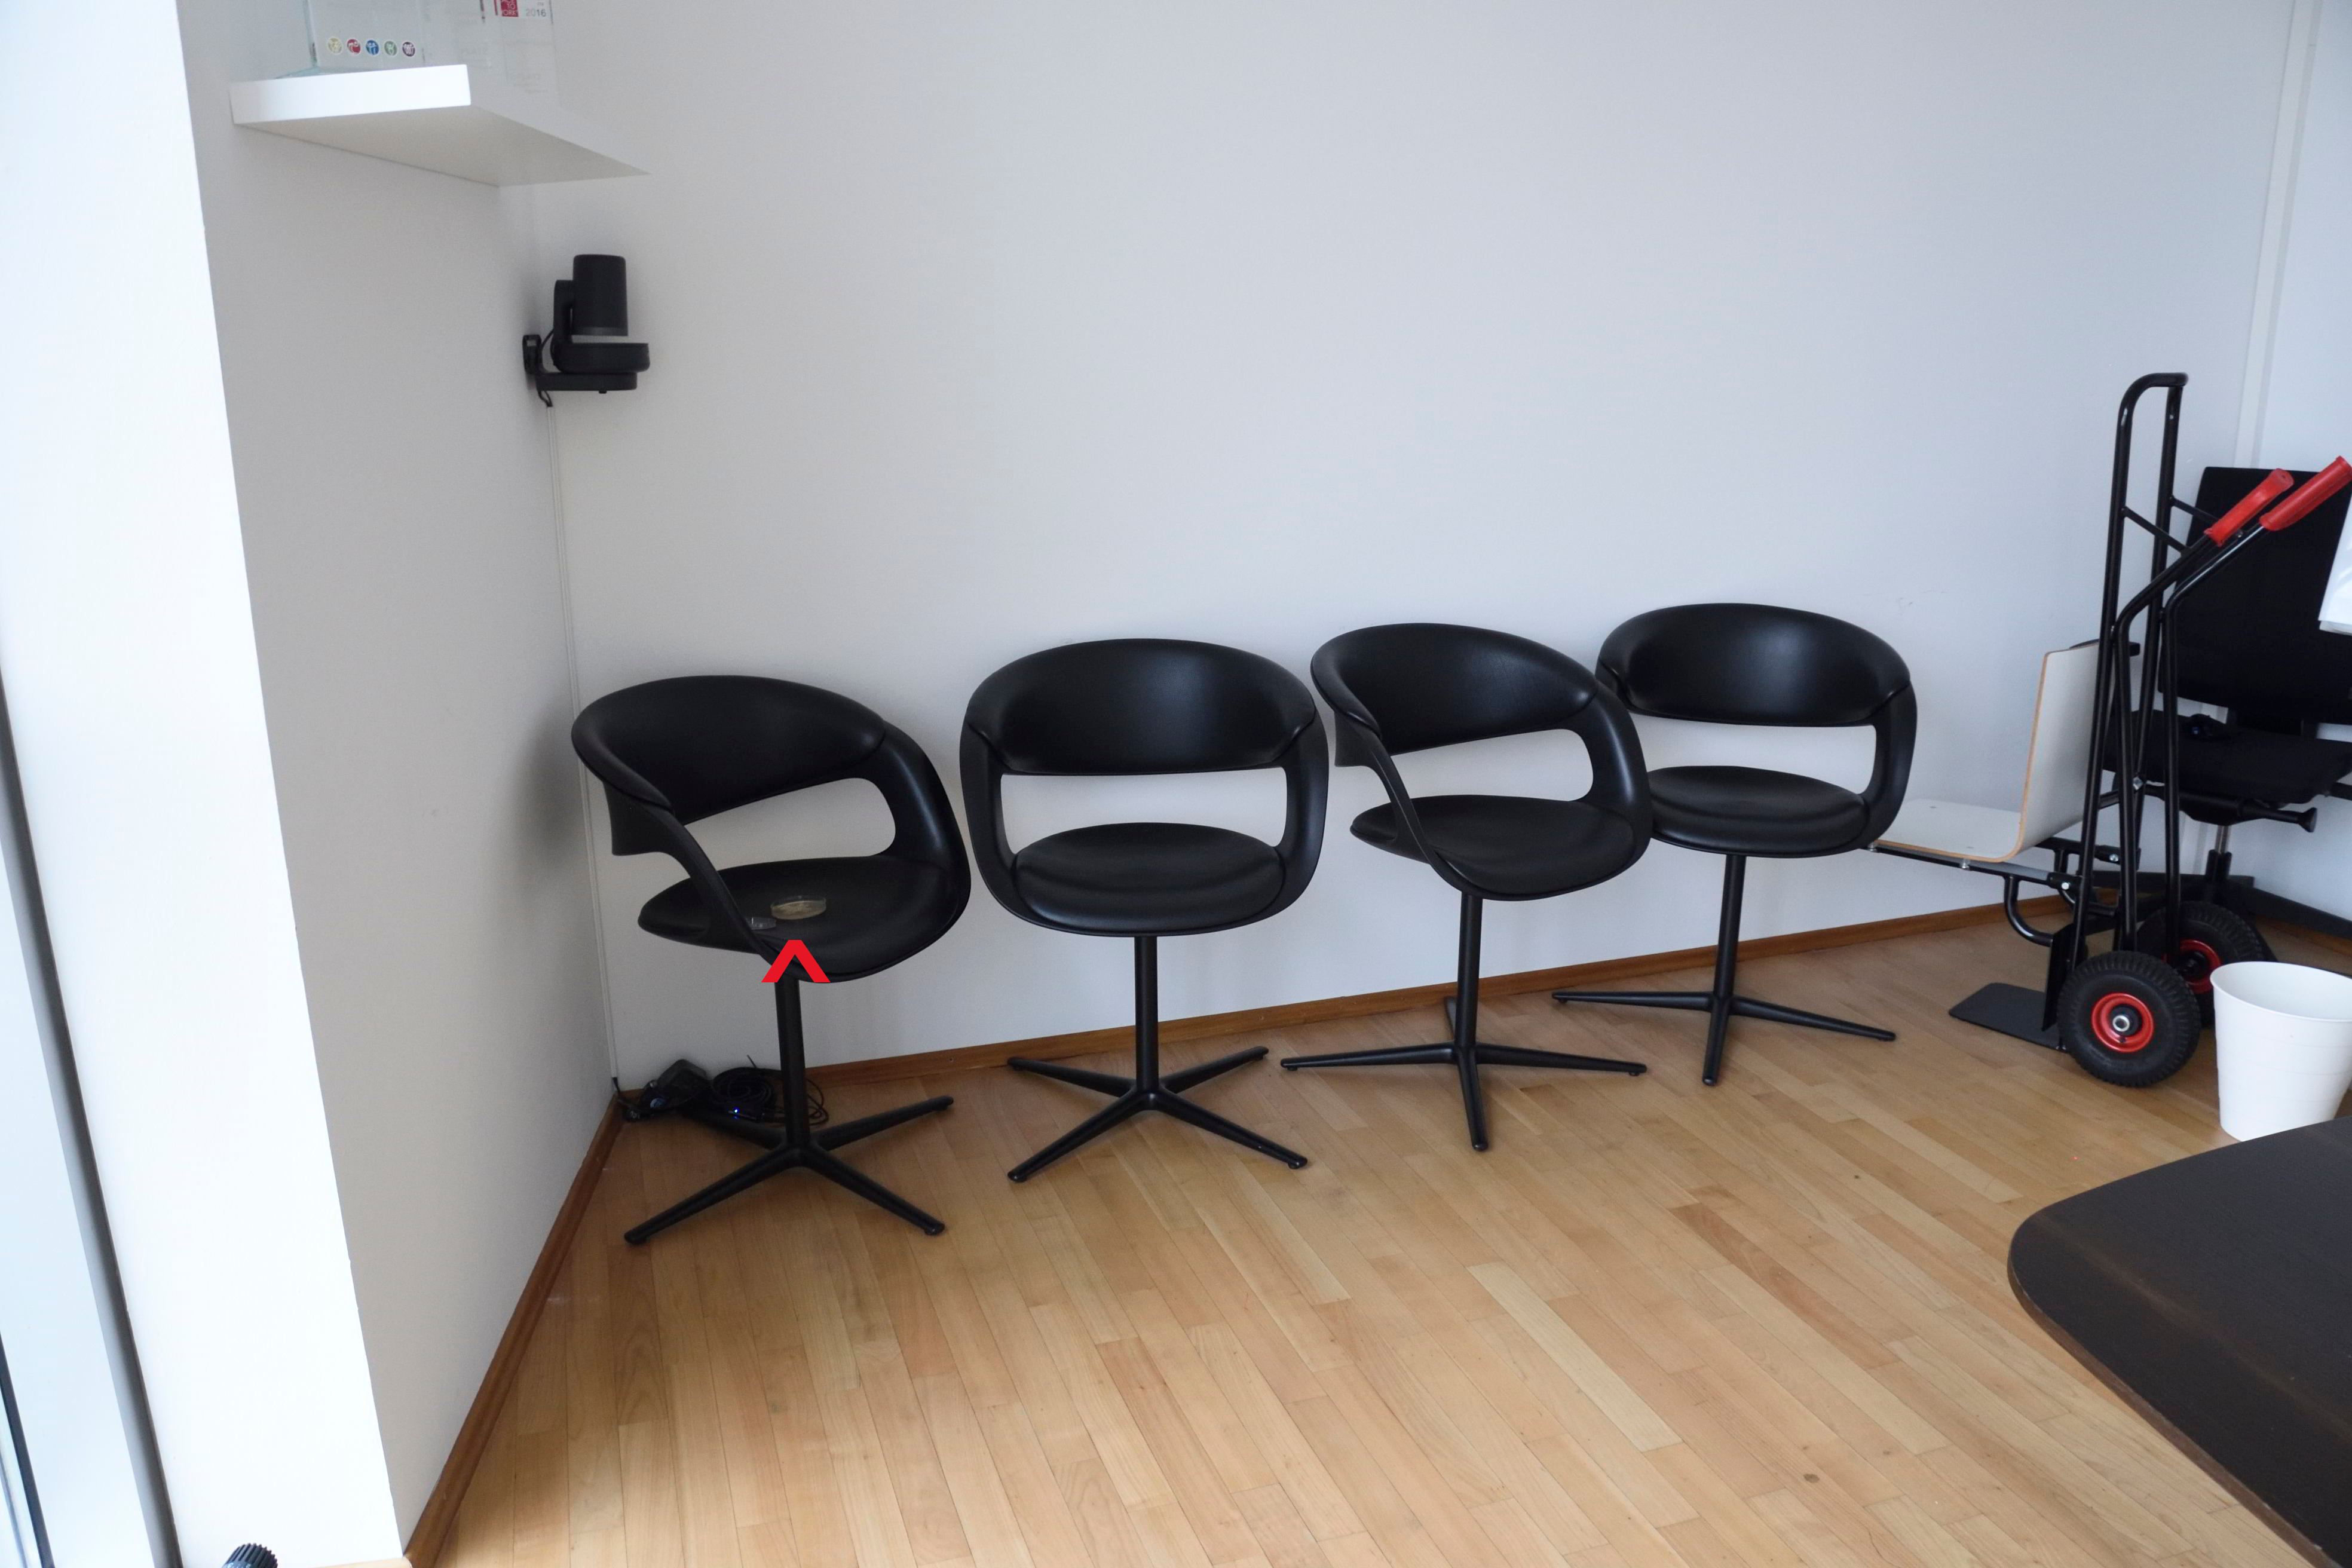
\includegraphics[scale=0.05]{_DSC7623}\hfill
\includegraphics[scale=0.05]{_DSC7624}\\
\includegraphics[scale=0.05]{_DSC7621}\\
\caption{photos showing the office and the placement of the CleanAir device and agar plates (red arrows)}
\end{figure*}
\end{document}